% !TEX encoding = UTF-8 Unicode
% !TEX spellcheck = en-US


% This is the root file of your thesis: thesis.tex
% A line starting with % is a comment. In some cases, I have included a command preceded by a %. You may activate the command by removing the %.

%%===================================
\documentclass[12pt]{report}
\usepackage{ramsstyle}
%%===================================
%Write the various parts of your thesis as separate files and include them into the main file by the command \include{name of included file}. When you compile the LaTeX file, you may choose which subfiles to include by the command

%\includeonly{chapter01,chapter02}
%\usepackage{amsmath}
\usepackage{algorithmic}
\usepackage{algorithm}
\usepackage{amssymb}
\usepackage{graphicx}
\usepackage{caption}
\usepackage{subcaption}
\usepackage{mathtools}

%%===================================
\begin{document}
% !TEX encoding = UTF-8 Unicode
%!TEX root = thesis.tex
% !TEX spellcheck = en-US

%This is the Titlepage
%%=========================================
\thispagestyle{empty}

\includegraphics[height=0.6in]{fig/rams}
\mbox{}\\[6pc]
\begin{center}
\Huge{A Krylov projection method for the heat equation }\\[2pc]

\Large{Sindre Eskeland}\\[1pc]
\large{\today}\\[2pc]

PROJECT\\
Department of Mathematical Sciences\\
Norwegian University of Science and Technology
\end{center}
\vfill

\noindent Supervisor: Professor Elena Celledoni

%\noindent Supervisor 2: Professor Fingal Olsson

 % This is the titlepage
\setcounter{page}{0}
\pagenumbering{roman}
% !TEX encoding = UTF-8 Unicode
%!TEX root = thesis.tex
% !TEX spellcheck = en-US
%%=========================================
\addcontentsline{toc}{section}{Preface}
\section*{Preface}
This is a project thesis as a part of the study program industrial mathematics. It was written during the summer of 2015. 
It is assumed that the reader is known with numerical difference methods and numerical linear algebra.

%Here, you give a brief introduction to your work. What it is (e.g., a Master's thesis in RAMS at NTNU as part of the study program xxx and\ldots), when it was carried out (e.g., during the autumn semester of 2021). If the project has been carried out for a company, you should mention this and also describe the cooperation with the company. You may also describe how the idea to the project was brought up.

%You should also specify the assumed background of the readers of this report (who are you writing for).\\[2cm]

%\begin{center}
%Trondheim, 2012-12-16\\[1pc]
%(Your signature)\\[1pc]
%Ola Nordmann
%\end{center}
% !TEX encoding = UTF-8 Unicode
%!TEX root = thesis.tex
% !TEX spellcheck = en-US
%%=========================================
\addcontentsline{toc}{section}{Acknowledgment}
\section*{Acknowledgment}
Thanks to Elena Celledoni for guiding me.%, and giving me the notes\cite{elena} I have shamelessly copied without referencing.
%\begin{flushright}
%O.N.\\[1pc]
%(Your initials)
%\end{flushright}
% !TEX encoding = UTF-8 Unicode
%!TEX root = thesis.tex
% !TEX spellcheck = en-US
%%=========================================
\addcontentsline{toc}{section}{Summary and Conclusions}
\section*{Summary and Conclusions}
Solving partial differential equations with finite difference methods often requires performing operations on huge linear systems. The Krylov projection method allows the user to choose the size of the linear system by making the method iterative. The Krylov projection method was tested on the heat equation against other methods in convergence, memory demand and computation time. The results shows that the Krylov projection method can reduce memory demand, and computation time if several processing units is used or some assumptions are met. No difference regarding convergence was found.
\tableofcontents
\setcounter{page}{0}
%\setcounter{section}{1}
\pagenumbering{arabic}
%%%%%%%%%%%%%%%%%%%%%%%%%%%%%%%%%%%%%%%%%%%%%%%%%%%%%%%%%%%%%%%%%%%%%%%%%%%%%%%%%%%%%%%%%%%%%%%%%%%%%%%%%%%%%%%%%%%%%%
\chapter{Introduction}%%%%%%%%%%%%%%%%%%%%%%%%%%%%%%%%%%%%%%%%%%%%%%%%%%%%%%%%%%%%%%%%%%%%%%%%%%%%%%%%%%%%%%%%%%%%%%
%%%%%%%%%%%%%%%%%%%%%%%%%%%%%%%%%%%%%%%%%%%%%%%%%%%%%%%%%%%%%%%%%%%%%%%%%%%%%%%%%%%%%%%%%%%%%%%%%%%%%%%%%%%%%%%%%%%%%%

In this text we will investigate how well the Krylov projection method (KPM) can be used to solve linear differential equations in the form $q'(t)=Aq(t)+f(t)$. These problems arise for example when discretizing time dependent, linear partial differential equations with the method of lines, and have therefore a wide range of applications. 
KPM is an orthogonal projection technique, the method is explained in detail in section \ref{sec:krylov}. We use Arnoldi's method which allows us to construct an orthonormal basis for a given Krylov subspace, this gives rise to two slightly different methods, presented in detail in section \ref{sec:fullKPM} and \ref{sec:rest} respectively.

The main focus of this report is to solve the heat equation with KPM, and compare convergence and computation time with an alternative solution technique, the alternative will be presented in section \ref{sec:DM}.
We state the heat equation here with boundary conditions for future references. \\
\begin{equation} \label{eqn:heat}
\begin{aligned}
\frac{\partial u(t,x,y)}{\partial t} - \nabla^2 u(t,x,y) &= p(t,x,y) & t \in [0,T]\\
u(0,x,y) &= 0 \\
u & = 0 			&\text{ on } \partial [0,L] \times [0,L]
\end{aligned}
\end{equation}
$p(t,x,y)$ is a smooth function, and $u(t,x,y)$ is the solution we seek.\\

Let us for now assume that the right hand side of equation \eqref{eqn:heat} is separable, so that $p(t,x,y) = f(t)g(x,y) $. 
Given a vector $v = [v_1,v_2, \cdots, v_m] \in \mathbb{R}^m $ with elements $ g(x_i,y_j)$, $x_i,y_j \in [0,L]$ and a matrix $A$ as an approximation of the Laplacian, we can write the heat equation on the form


\begin{equation} \label{eqn:numheat}
\begin{aligned}
q'(t) -Aq(t) &= f(t) v, \qquad & t \in [0,T] \\
q(0) &= 0               
\end{aligned}
\end{equation}
where $A$ is an $m \times m$ matrix assumed to be time independent, $f(t)$ is continuous on $[0,T]$, $v \in \mathbb{R}^m$, $q(t)$ is the unknown vector, for $t \in [0,T]$. Note also that $f(t)$ is a scalar function, so that $f(t) v = [f(t)v_1,f(t)v_2, \cdots,f(t) v_m] $.
The solution is 
\begin{equation}
q(t) = \int \limits_0^t \exp(A(t-s))f(s)v ds
\end{equation}
More details about $A$, $x_i$, $y_i$ and $q(t)$ will be given in section \ref{sec:imp}.

%%%%%%%%%%%%%%%%%%%%%%%%%%%%%%%%%%%%%%%%%%%%%%%%%%%%%%%%%%%%%%%%%%%%%%%%%%%%%%%%%%%%%%%%%%%%%%%%%%%%%%%%%%%%%%%%%%%%%%
\chapter{Krylov subspace and methods}%%%%%%%%%%%%%%%%%%%%%%%%%%%%%%%%%%%%%%%%%%%%%%%%%%%%%%%%%%%%%%%%%%%%%%%%%%%%%%%%
%%%%%%%%%%%%%%%%%%%%%%%%%%%%%%%%%%%%%%%%%%%%%%%%%%%%%%%%%%%%%%%%%%%%%%%%%%%%%%%%%%%%%%%%%%%%%%%%%%%%%%%%%%%%%%%%%%%%%%
%This section will be concerned with deriving KPM.
\label{sec:krylov}
In this chapter some solution techniques will be derived.
The Krylov subspace will be presented in section \ref{sec:subspace}, KPM will be derived for the heat equation in section \ref{sec:fullKPM} and \ref{sec:rest}. In section \ref{sec:nonsep} it is show how KPM can be used when $p$ is not separable. The method we will compare KPM to will be introduced in section \ref{sec:DM}. 
 %in section \ref{sec:nonsep}.


%%%%%%%%%%%%%%%%%%%%%%%%%%%%%%%%%%%%%%%%%%%%%%%%%%%%%%%%%%%%%%%%%%%%%%%%%%%%%%%%%%%%%%%%%%%%%%%%%%%%%%%%%%%%%%%%%%%%%%
\section{Krylov subspace} \label{sec:subspace}
%%%%%%%%%%%%%%%%%%%%%%%%%%%%%%%%%%%%%%%%%%%%%%%%%%%%%%%%%%%%%%%%%%%%%%%%%%%%%%%%%%%%%%%%%%%%%%%%%%%%%%%%%%%%%%%%%%%%%%
The Krylov subspace is the space $W_n (A,v) = \{v,Av, \cdots, A^{n-1}v\} = \{v^1,v^2,\cdots,v^n\} $, where $n \leq m$. %Define $\nu$ as the $W_\nu(A,v)$ span $A$. 
The vectors $v^i$ together with $h_{i,j} = v^i^\top Av^j$, are found by using Arnoldi's algorithm, shown in algorithm \ref{alg:arnoldi}. Letting $V_n$ be the $m \times n$ matrix consisting of column vectors $\{v^1,v^2,\cdots,v^n \}$ and $H_n$ be the $n \times n$ upper Hessenberg matrix containing all elements $(h_{i,j})_{i,j=1,\cdots,n}$, the following holds \cite{saad}
\begin{align}\
AV_n & = V_n H_n + h_{n+1,n}v_{n+1}e^\top_n \label{eqn:prop1} \\
V^{\top}_n AV_n &= H_n \label{eqn:prop2} \\
v^i^{\top} v^j &= \delta_{i,j}. \label{eqn:prop3}
\end{align}
Here, $e_n$ is the $n$th canonical vector in $\mathbb{R}^n$ and $\delta_{i,j}$ is Kronecker's delta.\\




\begin{algorithm} 
\begin{algorithmic} \caption{Arnoldi's algorithm\cite{saad}} \label{alg:arnoldi}  
\STATE Start with $A$, $v^1 = v/\|v \|_2$ and $n$
\FOR{$j = 1,2,\cdots n $} 
   \STATE Compute $h_{i,j} = \langle Av^j,v^i \rangle $ for $i = 1,2,\cdots j$
    \STATE Compute $w_j := A v^j - \Sigma_{i=1}^{j} h_{i,j}v^i $
    \STATE $h_{j+1,j} = \| w_j \|_2$
    \IF{$h_{j+1,j} = 0$} 
        \STATE\textbf{STOP}
    \ENDIF 
   \STATE $v^{j+1} = w_j/h_{j+1,j}$
\ENDFOR
\end{algorithmic} 
\end{algorithm}
%Let us assume that $\nu \leq m$ is the index such that $W_v(A,v)=\mathbb{R}^m$.
%Let us define $\nu  \leq m$ as the constant where $W_\nu(A,v)$ spans $A$, meaning we run Arnoldi's algorithm until the stopping criterium is met.
%%%%%%%%%%%%%%%%%%%%%%%%%%%%%%%%%%%%%%%%%%%%%%%%%%%%%%%%%%%%%%%%%%%%%%%%%%%%%%%%%%%%%%%%%%%%%%%%%%%%%%%%%%%%%%%%%%%%%%
\section{Krylov projection method} \label{sec:fullKPM}
%%%%%%%%%%%%%%%%%%%%%%%%%%%%%%%%%%%%%%%%%%%%%%%%%%%%%%%%%%%%%%%%%%%%%%%%%%%%%%%%%%%%%%%%%%%%%%%%%%%%%%%%%%%%%%%%%%%%%%

Let $z(t) = [z_1(t), z_2(t), \cdots, z_m(t)] \in \mathbb{R}^m $ be the vector satisfying $q(t) = V_m z(t)$, where $q(t)$ is from equation \eqref{eqn:numheat}, and $V_m$ is obtained by running algorithm \ref{alg:arnoldi} with $n = m$. 
We derive KPM by writing this into \eqref{eqn:numheat}, that is
\begin{equation*}  \begin{aligned} \label{eqn:KPMtemp1}
V_m z'(t) - A V_m z(t) &= f(t) v \\
z(0)& = 0.
\end{aligned} \end{equation*}
Multiplying by $V_m^{\top}$ and using equation \eqref{eqn:prop2} gives
\begin{equation*} 
\begin{aligned} \label{eqn:KPMtemp2}
z'(t)-H_m z(t) &= f(t) V_m^{\top}  v  \\
z(0)& = 0.
\end{aligned}
\end{equation*}
Using equation \eqref{eqn:prop3} and $v = \|v \|_2 v^1 $, we get
\begin{equation} 
\begin{aligned} \label{eqn:krylov}
z'(t) -H_m z(t) &=  \|v \|_2 e_1 f(t)\\
z(0)& = 0.
\end{aligned}
\end{equation}
By solving equation \eqref{eqn:krylov} for $z(t)$ and calculating $ q(t) = V_m z(t) $ the solution is obtained. A step by step description is given in algorithm \ref{alg:fullkry}. 
%\end{proof}
The method will be denoted KPM.\\
\begin{algorithm}
\begin{algorithmic} \caption{The Krylov projection method} \label{alg:fullkry} 
\STATE Start with $A$,$f(t)$ and $v$.
\STATE Compute $[V_m ,H_m] = \texttt{arnoldi}(A,v)$
\STATE Solve $  z'(t) = H_m z + f(t) \| v \|_2 e_1  $ for $z$
\STATE $ q_m (t) \leftarrow  V_m z(t) $
\end{algorithmic} 
\end{algorithm}

Consider the residual of equation \eqref{eqn:numheat} at $q_n(t) = V_n z (t)$, that is
\begin{equation*}
r_n(t) = f(t) v - q_n'(t) +Aq_n(t).
\end{equation*}
Since
\begin{equation*}
r_n(t) = f(t)v -V_n z'(t) + A V_n z(t)
\end{equation*}
using equation \eqref{eqn:prop1} and \eqref{eqn:krylov} we get
\begin{equation} \label{eqn:rn}
r_n(t) = h_{n+1,n}e_n^\top z(t) v_{n+1}.
\end{equation}

Since $h_{n+1,n} = 0$ for some $n \leq m$, this shows the finite termination of the procedure.


%%%%%%%%%%%%%%%%%%%%%%%%%%%%%%%%%%%%%%%%%%%%%%%%%%%%%%%%%%%%%%%%%%%%%%%%%%%%%%%%%%%%%%%%%%%%%%%%%%%%%%%%%%%%%%%%%%%%%%
\section{Restarting the Krylov projection method} \label{sec:rest}
%%%%%%%%%%%%%%%%%%%%%%%%%%%%%%%%%%%%%%%%%%%%%%%%%%%%%%%%%%%%%%%%%%%%%%%%%%%%%%%%%%%%%%%%%%%%%%%%%%%%%%%%%%%%%%%%%%%%%%
If $n < m$ so that $h_{n+1,n} \neq 0$, we need to restart the procedure described above. Consider first the following equation
\begin{equation}\label{eqn:restkry}
\begin{aligned}
 (q-q_n)'(t) -A (q-q_n)(t) &= r_n \\
(q-q_n)(0)& = 0
\end{aligned}
\end{equation}
where $r_n$ is as in equation \eqref{eqn:rn}. Solving this equation for $(q-q_n)$, can improve the approximation of $q$ via iterative refinement.
Equation \eqref{eqn:restkry} is of the same form as equation \eqref{eqn:krylov}. We derive KPM as before, by writing $q(t) = V_m z(t)$ and $q_n = \tilde{V}_n \tilde{\zeta} $. Let $\tilde{V}_n$ be the $m \times m$ matrix with the first $n$ columns equal to the first $n$ columns of $V_m$, and all additional elements equal to zero. The first $n$ rows of  $\tilde{\zeta}$ is equal to $\zeta$, where $q_n = V_n \zeta$. The rest of the elements in $\tilde{\zeta}$ are equal to zero.
We then get
\begin{equation*}
\begin{aligned}
 (V_m z-\tilde{V}_n \tilde{\zeta})'(t)-A (V_m z-\tilde{V}_n \tilde{\zeta})(t) &=  h_{n+1,n}e_n^\top \tilde{\zeta}(t) v^{n+1}  \\
(z-\tilde{\zeta})(0)& = 0 .
\end{aligned}
\end{equation*}
Multiplying by $V_m^{\top}$ and using equation \eqref{eqn:prop2} gives
\begin{equation*}
\begin{aligned}
 (z-\tilde{\zeta})'(t)-\tilde{H_n} (z-\tilde{\zeta})(t) &= V_m^\top h_{n+1,n}e_n^\top \tilde{\zeta}(t) v^{n+1}  \\
(z-\tilde{\zeta})(0)& = 0.
\end{aligned}
\end{equation*}
Let $\tilde{\xi}(t) = (z-\tilde{\zeta})(t)$, and simplify
\begin{equation*} 
\begin{aligned}
 \tilde{\xi} '(t) -\tilde{H_n} \tilde{\xi}(t) &= h_{n+1,n}e_n^\top \tilde{\zeta} (t)  \\
\tilde{\xi}(0)& = 0.
\end{aligned}
\end{equation*}
Drop all except the $n$ first rows of $\tilde{\xi}(t)$, and we are left with
\begin{equation}\label{eqn:restkry2}
\begin{aligned}
 \xi '(t) -H_n \xi(t) &= h_{n+1,n}e_n^\top \zeta (t)  \\
\xi(0)& = 0.
\end{aligned}
\end{equation}

Each restart we generate a new Krylov subspace $W_n(A,v^{n+1})$, solve equation \eqref{eqn:restkry2} for $\xi(t)$ and approximate the solution $q$ by $ q_n =  V_n\xi(t)$. By summing together $q_n$, we converge towards $q$. Note that the current value of $\zeta(t)$ equals the previous value of $\xi(t)$, and that $h_{n+1,n}$ is from the previous $H_n$. See algorithm \ref{alg:restkry} for a step by step description. We will call $n$ a restart variable, and denote the method with KPM$(n)$.
\begin{algorithm}
\begin{algorithmic} \caption{The Krylov projection method with restart} \label{alg:restkry} 
\STATE Start with $A$,$f(t)$,$v$, $n$ and $i = 0$
\STATE Compute $[V_n,H_n,h_{n+1,n}^i,v^{n+1}] = \texttt{arnoldi}(A,v)$
\STATE Solve $  z' = H_n z + f(t) \| v \|_2 e_1  $ for $z$
\STATE $ q_n \leftarrow  V_n z $
\STATE $\xi_i \leftarrow z$
\WHILE{convergence criterion not satisfied} 
    \STATE $i \leftarrow i + 1$
    \STATE Compute $[V_n,H_n,h_{n+1,n}^i,v^{n+1}] = \texttt{arnoldi}(A,v^{n+1},n)$
    \STATE Solve $ \xi_i'(t) = H_n \xi_i(t) + h_{n+1,n}^{i-1}e_n^\top \xi_{i-1}(t)  $ for $\xi_i$
    \STATE $ q_n(t) \leftarrow q_n + V_n \xi_i(t) $
\ENDWHILE
\end{algorithmic} 
\end{algorithm}

%%%%%%%%%%%%%%%%%%%%%%%%%%%%%%%%%%%%%%%%%%%%%%%%%%%%%%%%%%%%%%%%%%%%%%%%%%%%%%%%%%%%%%%%%%%%%%%%%%%%%%%%%%%%%%%%%%%%%%
\section{When $p$ is not seperable} \label{sec:nonsep}
%%%%%%%%%%%%%%%%%%%%%%%%%%%%%%%%%%%%%%%%%%%%%%%%%%%%%%%%%%%%%%%%%%%%%%%%%%%%%%%%%%%%%%%%%%%%%%%%%%%%%%%%%%%%%%%%%%%%%%
Let $P(t)$ be a vector consisting of elements $p(t, x_i, y_j)$, so that $P(t) = [P_1(t),P_2(t),\cdots, P_m(t)]$. Writing equation \eqref{eqn:numheat} as

\begin{equation}
\begin{aligned}
q'_j(t) -A q_j(t) &= P_j(t) e_j \\
q_j(0) &= 0\\
q(t) &= \sum \limits_{i = 1}^m q_j(t),
\end{aligned}
\end{equation}
where $e_j$ is the $j$th canonical vector in $\mathbb{R}^{m}$, we can then solve the original equation without requiring separability. 
An important thing to note here is the need for parallel processing power, since $m$ problems must be solved and not just one.
%%%%%%%%%%%%%%%%%%%%%%%%%%%%%%%%%%%%%%%%%%%%%%%%%%%%%%%%%%%%%%%%%%%%%%%%%%%%%%%%%%%%%%%%%%%%%%%%%%%%%%%%%%%%%%%%%%%%%%
\section{Direct method} \label{sec:DM}
%%%%%%%%%%%%%%%%%%%%%%%%%%%%%%%%%%%%%%%%%%%%%%%%%%%%%%%%%%%%%%%%%%%%%%%%%%%%%%%%%%%%%%%%%%%%%%%%%%%%%%%%%%%%%%%%%%%%%%
Since the objective of this report is to measure how KPM performs, we need something to compare it to. For this, solve 
\begin{equation} \label{eqn:DI}
q'(t) -A q(t) = P(t)
\end{equation}
for $q(t)$, without using KPM. Let $P(t)$ be as in section \ref{sec:nonsep} and denote the method DM for direct method.
%\newpage
%%%%%%%%%%%%%%%%%%%%%%%%%%%%%%%%%%%%%%%%%%%%%%%%%%%%%%%%%%%%%%%%%%%%%%%%%%%%%%%%%%%%%%%%%%%%%%%%%%%%%%%%%%%%%%%%%%%%%%
\chapter{Implementation}%%%%%%%%%%%%%%%%%%%%%%%%%%%%%%%%%%%%%%%%%%%%%%%%%%%%%%%%%%%%%%%%%%%%%%%%%%%%%%%%%%%%%%%%%%%%%%
%%%%%%%%%%%%%%%%%%%%%%%%%%%%%%%%%%%%%%%%%%%%%%%%%%%%%%%%%%%%%%%%%%%%%%%%%%%%%%%%%%%%%%%%%%%%%%%%%%%%%%%%%%%%%%%%%%%%%%
\label{sec:imp}
This section will explain the implementation of the methods. We start by discretization in space and time in section \ref{sec:space} and \ref{sec:time} respectively, and introduce the method we will compare KPM to in section \ref{sec:DM}. 
In section \ref{sec:not} we present what and how we want to measure interesting factors, together with some information about computers and programs used to generate data.
In section \ref{sec:test} we state some test problems.

%%%%%%%%%%%%%%%%%%%%%%%%%%%%%%%%%%%%%%%%%%%%%%%%%%%%%%%%%%%%%%%%%%%%%%%%%%%%%%%%%%%%%%%%%%%%%%%%%%%%%%%%%%%%%%%%%%%%%%
\section{Discretisation in space} \label{sec:space}
%%%%%%%%%%%%%%%%%%%%%%%%%%%%%%%%%%%%%%%%%%%%%%%%%%%%%%%%%%%%%%%%%%%%%%%%%%%%%%%%%%%%%%%%%%%%%%%%%%%%%%%%%%%%%%%%%%%%%%
We consider the square $[0,1] \times [0,1]$ and divide each spacial direction into $\rho+2$ piece, each piece having a length of $h_s = 1/(\rho+1)$. Let $x_i = h_s \cdot i$ and $y_i = h_s \cdot j$ . Since the boundary conditions are known, we will only calculate with $\rho$ numbers, leaving room on each side for the boundary. $v$ and $P(t)$ need to be found in an ordered fashion. We let  $v_{i+\rho j} = g(x_i, y_j)$, and 
$P(t)_{i+\rho j} = p(t,x_i, y_j)$, where $i,j = 1,2,\cdots \rho+1$.
The Laplacian will be approximated by the five point formula given in equation \eqref{eqn:fivepoint} as the matrix $A$. This is a second order approximation.
\begin{equation} \label{eqn:fivepoint} 
\begin{aligned} 
A = \frac{1}{h_s^2} 
\begin{bmatrix}
T & I & & &\\
I& T & I & &\\
& \ddots & \ddots & \ddots & \\
& & I& T & I\\
& & & I & T
\end{bmatrix}
, T  &= 
\begin{bmatrix}
-4 & 1 & & &\\
1 & -4 & 1 & &  \\
& \ddots & \ddots & \ddots & \\
&  & 1 & -4 & 1 \\
 & & & 1 & -4
\end{bmatrix},
I &= 
\begin{bmatrix}
1 & &\\
& \ddots & \\
& & 1 \\
\end{bmatrix}
\end{aligned}
\end{equation}
Notice that $m = \rho ^2$.

%%%%%%%%%%%%%%%%%%%%%%%%%%%%%%%%%%%%%%%%%%%%%%%%%%%%%%%%%%%%%%%%%%%%%%%%%%%%%%%%%%%%%%%%%%%%%%%%%%%%%%%%%%%%%%%%%%%%%%
\section{Discretisation in time} \label{sec:time}
%%%%%%%%%%%%%%%%%%%%%%%%%%%%%%%%%%%%%%%%%%%%%%%%%%%%%%%%%%%%%%%%%%%%%%%%%%%%%%%%%%%%%%%%%%%%%%%%%%%%%%%%%%%%%%%%%%%%%%
We will consider the time domain $t \in [0,1] $, and divide it in $k$ pieces, giving each piece a length $h_t = 1/(k-1)$, let $t_l = h_t\cdot l$.
Trapezoidal rule\cite{trap}, given in equation \eqref{eqn:trap} will be used to integrate in time. 
\begin{equation} \label{eqn:trap}
\int \limits_a^b f(t) dt \approx \frac{h}{2} \sum \limits_{l = 1}^N(f(t_{l+1})+f((t_l))
\end{equation}
We will only derive the iteration scheme for equation \eqref{eqn:numheat}, but since all the differential equations are similar, it should be easy to make the few changes necessary to solve the other differential equations discussed.
To obtain the iteration scheme we write $q$ instead of $f$, use equation \eqref{eqn:heat} and insert the numerical simplifications above.
\begin{equation}
q(t_{l+1}) - q(t_l) = \int \limits_{t_l}^{t_{l+1}} \frac{\partial q}{\partial t} dt \approx \frac{h}{2}(A q(t_{l+1})+f(t_{l+1})v +A q(t_l)+f(t_l) v) 
\end{equation}
Solving for $q(t_{l+1})$ gives the Crank-Nicholson scheme for the heat equation.
\begin{equation} \label{eqn:trapscheme}
\begin{aligned}
q(t_{l+1}) \approx (I-h_t/2 A)^{-1}(q(t_l) + \frac{h_t}{2}( A q(t_{l}) + f(t_l)v+f(t_{l+1})v))\\
%U^{l+1} = (I-h_t/2 A)^{-1}(U^l + \frac{h_t}{2}( A U^l + G^l+G^{l+1}))
\end{aligned}
\end{equation} 
This is a second order method.
%%%%%%%%%%%%%%%%%%%%%%%%%%%%%%%%%%%%%%%%%%%%%%%%%%%%%%%%%%%%%%%%%%%%%%%%%%%%%%%%%%%%%%%%%%%%%%%%%%%%%%%%%%%%%%%%%%%%%%
\section{Direct method} \label{sec:DM}
%%%%%%%%%%%%%%%%%%%%%%%%%%%%%%%%%%%%%%%%%%%%%%%%%%%%%%%%%%%%%%%%%%%%%%%%%%%%%%%%%%%%%%%%%%%%%%%%%%%%%%%%%%%%%%%%%%%%%%
We need to compare KPM to a well known and easy to implement method. For this we will solve equation \eqref{eqn:DI} straight forward with trapezoidal rule.
\begin{equation} \label{eqn:DI}
q'(t) -A q(t) = P(t)
\end{equation}
We denote it DM for direct method.
\newpage
%%%%%%%%%%%%%%%%%%%%%%%%%%%%%%%%%%%%%%%%%%%%%%%%%%%%%%%%%%%%%%%%%%%%%%%%%%%%%%%%%%%%%%%%%%%%%%%%%%%%%%%%%%%%%%%%%%%%%%
\section{Measurements and computers} \label{sec:not}
%%%%%%%%%%%%%%%%%%%%%%%%%%%%%%%%%%%%%%%%%%%%%%%%%%%%%%%%%%%%%%%%%%%%%%%%%%%%%%%%%%%%%%%%%%%%%%%%%%%%%%%%%%%%%%%%%%%%%%

We divide implementations in two cases, separable $p$, and non separable $p$. Parallel computations were only implemented for non separable $p$. For both cases three solvers were implemented: KPM, KPM$(n)$, and DM. \\

The convergence criterium used in algorithm \ref{alg:restkry} is to stop when the maximum absolute difference in $q_n$ is less than a given tolerance $\delta$. The error is denoted as $\epsilon$ and is defined as the largest absolute difference between the correct solution and the approximation. 
The number of iterations needed for convergence in algorithm \ref{alg:restkry} is denoted by $\gamma$. 
We will in general be looking at computation time and error, and how this scale with $\delta$. \\

If nothing else is stated assume $\rho = k = 40$, $n = 1$, $\delta = 10^{-15}$. All timed results are averaged over 2 runs, preferably this should have been higher, but that was too time consuming. $A$ was implemented as a sparse matrix\\


All solvers and problems were implemented in MATLAB R2014b. The computer used runs Ubuntu 14.04 LTS with intel  i7-4770 CPU, and 16 GB ram. \\

The parallel implementations were done with MATLAB's commands \texttt{parpool} and \texttt{parfor}, see \cite{parpool} and \cite{parfor} for more information, \texttt{nP} denotes the number of processing units used. We will use speedup and parallel efficiency to investigate the gain by using parallel computation. Speedup is defined as
\begin{align*}
S_\texttt{nP} = \frac{\tau_1}{\tau_\texttt{nP}}
\end{align*}
and parallel efficiency as
\begin{align*}
\eta_\texttt{nP} = \frac{S_\texttt{nP}}{\texttt{nP}}
\end{align*}
where $\tau_\texttt{nP}$ is run time with \texttt{nP} processors, $S_\texttt{nP}$ is speedup with \texttt{nP} processors, and $\eta_\texttt{nP}$ is parallel efficiency for \texttt{nP} processors. Speedup measures how much faster a program runs with \texttt{nP} processors, ideal speedup is when $S_\texttt{nP} = \texttt{nP}$. Parallel efficiency measures how well each processor is used. Perfect parallel efficiency occurs when $\eta_\texttt{nP} = 1$.
%%%%%%%%%%%%%%%%%%%%%%%%%%%%%%%%%%%%%%%%%%%%%%%%%%%%%%%%%%%%%%%%%%%%%%%%%%%%%%%%%%%%%%%%%%%%%%%%%%%%%%%%%%%%%%%%%%%%%%
\section{Test problems} \label{sec:test}
%%%%%%%%%%%%%%%%%%%%%%%%%%%%%%%%%%%%%%%%%%%%%%%%%%%%%%%%%%%%%%%%%%%%%%%%%%%%%%%%%%%%%%%%%%%%%%%%%%%%%%%%%%%%%%%%%%%%%%
Two test problems are implemented for the separable case. Equation \eqref{eqn:sep1} is a symmetric problem, and separable for each variable, we will denote it as \texttt{P1}. 
\begin{equation} \label{eqn:sep1}
\begin{aligned}
 u(t,x,y)&= \frac{t}{t+1} x(x-1)y(y-1) \\
 f_1(t)&=\frac{1}{t+1^2} & g_1(x,y)&= x(x-1)y(y-1) \\
 f_2(t) &= \frac{-t}{t+1} & g_2(x,y)& = 2x(x-1) +2y(y-1)
 \end{aligned}
\end{equation}
Equation \eqref{eqn:sep2} is not symmetric, and non separable for $x$ and $y$, it also has a combination of polynomials and exponential functions, just to make it test a more general case. 
This problem will be denoted as \texttt{P2}.\\
\begin{equation} \label{eqn:sep2}
\begin{aligned}
 u(t,x,y)=& e^{xy}y(y-1) \sin( \pi x)t \cos(t)& \\
 f_1(t) =& \cos(t)-t \sin(t)  & g_1(x,y) =&e^{xy}y(y-1) \sin( \pi x)\\
 f_2(t) =& -t \cos(t) \\ g_2(x,y) =&(y-1)y^3e^{xy} \sin ( \pi x)
 \end{aligned}
\end{equation}
\begin{equation*}
\begin{aligned}
&+e^{xy}(x^2(y-1)y+x(4y-2)+2) \sin( \pi x) \\&+2 \pi (y-1) y^2 e^{xy} \cos( \pi x)- \pi^2 (y-1)y e^{xy} \sin( \pi x )
 \end{aligned}
\end{equation*}

To obtain the solutions, we need to solve for $f_i(t) g_i(x,y)$, $i = 1,2 $ and add the solutions together. Clearly parallel computations could be used to solve these, but this will not be done in this text. \\

\texttt{P1} will also be used in the non separable case with $p(t) = f_1(t) g_1(x,y) + f_2(t) g_2(x,y)$.
One additional test problem is implemented for non separable $p$, this is a symmetric problem consisting of both polynomial and exponential functions, it is given in equation \eqref{eqn:non1}, and will be denoted as \texttt{P3}.
\begin{equation} \label{eqn:non1}
\begin{aligned}
 u(t,x,y) = & \sin(x y t) (x-1) (y-1)\\
 p(t,x,y) = & t^2 (x-1) (y-1) y^2 \sin(t x y)\\ & -2 t (y-1) y \cos(t x y)+(x-1) x (y-1) y \cos(t x y)\\ & -t (x-1) x (2 \cos(t x y)-t x (y-1) \sin(t x y))
\end{aligned}
\end{equation}
%%%%%%%%%%%%%%%%%%%%%%%%%%%%%%%%%%%%%%%%%%%%%%%%%%%%%%%%%%%%%%%%%%%%%%%%%%%%%%%%%%%%%%%%%%%%%%%%%%%%%%%%%%%%%%%%%%%%%%
\chapter{Computational complexity}%%%%%%%%%%%%%%%%%%%%%%%%%%%%%%%%%%%%%%%%%%%%%%%%%%%%%%%%%%%%%%%%%%%%%%%%%%%%%%%%%%%
%%%%%%%%%%%%%%%%%%%%%%%%%%%%%%%%%%%%%%%%%%%%%%%%%%%%%%%%%%%%%%%%%%%%%%%%%%%%%%%%%%%%%%%%%%%%%%%%%%%%%%%%%%%%%%%%%%%%%%
\label{sec:comp}
We will in section \ref{sec:cc} and \ref{sec:mr} briefly compare the computational and memory costs of the different methods discussed.% This will be presented  respectivly. 
%%%%%%%%%%%%%%%%%%%%%%%%%%%%%%%%%%%%%%%%%%%%%%%%%%%%%%%%%%%%%%%%%%%%%%%%%%%%%%%%%%%%%%%%%%%%%%%%%%%%%%%%%%%%%%%%%%%%%%
\section{Computational complexity} \label{sec:cc}
%%%%%%%%%%%%%%%%%%%%%%%%%%%%%%%%%%%%%%%%%%%%%%%%%%%%%%%%%%%%%%%%%%%%%%%%%%%%%%%%%%%%%%%%%%%%%%%%%%%%%%%%%%%%%%%%%%%%%%
\begin{table}[H]
\centering
\begin{tabular}{r | l}
 Matrix vector multiplication (full) & $\mathcal{O}(m^2)$ \cite{complex} \\
 Matrix vector multiplication (sparse) & $\mathcal{O}(m)$ \cite{complex} \\
 Matrix inversion  & $ \mathcal{O}(m^3)$ \cite{complex} \\
 Arnoldi's algorithm & $ \mathcal{O}(n^2 m)$ \cite{saad} \\
 Integration & $\mathcal{O}(k)$
\end{tabular}
\caption{Computational complexity for some operations. Dimension of the matrices is assumed to be $m \times m$ while $n$ is the restart variable and $k$ is the number of steps in time.}
\label{tab:runtime}
\end{table}
DM need to perform $k$ matrix vector multiplications with a sparse matrix, and one matrix inversion. \\

KPM and KPM$(n)$ needs to perform $k$ matrix vector multiplications with a full matrix, and one matrix inversion. KPM and KPM$(n)$ also need to run Arnoldi's algorithm. If $p$ is non separable, all these operations need to be done $m$ times. If $p$ is separable, one time i enough. KPM$(n)$ uses smaller matrices and vectors, with size $n$. This reduces the cost of these operations, but the method needs to restart, we denote the number of restarts KPM$(n)$ need to converge as $\gamma$. \\

An overview over the computational cost of these operations is given in table \ref{tab:runtime}. A list of asymptotic computational complexity for the methods is given in table \ref{tab:cc}.
\begin{table}[H]
\centering
\begin{tabular}{l | l l}

Method & Separable $p$ & Non separable $p$ \\
\hline
 DM & $\mathcal{O}(km+m^3)$ & $\mathcal{O}(km+m^3)$  \\
 KPM& $\mathcal{O}(km^2 +m^3)$ & $\mathcal{O}(km^3 +m^4)$ \\
 KPM$(n)$& $\mathcal{O}((kn^2 +n^2m+n^3)\gamma)$  & $\mathcal{O}((kn^2m +n^2m^2+n^3m)\gamma)$
\end{tabular}
\caption{Computational complexity for the methods discussed, $\gamma$ denotes the number of restarts needed to converge. Parallel computations will be done for non separable $p$.}
\label{tab:cc}
\end{table}

We assume that KPM$(m)$ and KPM has the same complexity, so that $\gamma = 1$ when $n = m$. We see that KPM and KPM$(n)$ has a much higher estimated complexity if $p$ is not separable, this is the reason we divide between the two cases. The advantage with DM is the stable performance.
%%%%%%%%%%%%%%%%%%%%%%%%%%%%%%%%%%%%%%%%%%%%%%%%%%%%%%%%%%%%%%%%%%%%%%%%%%%%%%%%%%%%%%%%%%%%%%%%%%%%%%%%%%%%%%%%%%%%%%
\section{Memory requirement} \label{sec:mr}
%%%%%%%%%%%%%%%%%%%%%%%%%%%%%%%%%%%%%%%%%%%%%%%%%%%%%%%%%%%%%%%%%%%%%%%%%%%%%%%%%%%%%%%%%%%%%%%%%%%%%%%%%%%%%%%%%%%%%%

\begin{table}[H]
\centering
\begin{tabular}{r|l}
 $A$    & $ \sim 10 m$ \\
 $q$    & $ m\times k$ \\
 $P$ & $ m \times k$ \\
 $f$ & $ k $ \\
 $v$    & $ m$ \\
 $V_n$  & $ m \times n $ \\
 $H_n$  & $ n \times n $  \\
 Inverted matrix, with size $m \times m$ & $m \times m$ \\
\end{tabular}
\caption{List over memory demanding variables. All variables are assumed to be discretized with $k$ points in time, and $m$ points in space.}
\label{tab:memreq}
\end{table}
DM need to store $A$, $q$ ,$P$, and an inverted matrix with size $m \times m$.\\

KPM and KPM$(n)$ needs to store $A$, $q$, $V_n$, $H_n$, and an inverted matrix, remember that for KPM $n = m$. If $p$ is separable we also need to store $v$ and $f$, if $p$ is non separable we need to store $P$ instead. \\

An overview over the memory demand for the different variables is given in table \ref{tab:memreq}. A list of memory demand for the different methods is given in table \ref{tab:mr}.

\begin{table}[H]
\centering
\begin{tabular}{l | l l}
Method & Separable $p$ & Non separable $p$ \\
\hline
DM & $m^2+2mk+10m$ & $m^2+2mk + 10 m$ \\
KPM & $mk+3m^2+11m+k$ & $2mk+3m^2+11m+k$ \\
KPM$(n)$ & $ mk +2n^2+k+11m+nm $ &  $ 2(mk + n^2)+k+11m+nm $
\end{tabular}
\caption{Memory requirements for the methods discussed. The values are not given asymptotically so that it is easier to distinguish between the different methods.}
\label{tab:mr}
\end{table}

%We see that KPM$(m)$ and KPM requires the same amount of memory.
%!!!!!!!!!!!!!!!!!!!!!!!!!liten diskusjon her?!!!!!!!!!!!!!!!!!!!!!!!!!\\
KPM and KPM$(m)$ has the same memory demand, which makes sense. For KPM$(1)$ the memory demand is proportional to $mk$, which is much lover than for the other methods. The difference between separable and non separable $p$ is much smaller than in section \ref{sec:cc}.
%%%%%%%%%%%%%%%%%%%%%%%%%%%%%%%%%%%%%%%%%%%%%%%%%%%%%%%%%%%%%%%%%%%%%%%%%%%%%%%%%%%%%%%%%%%%%%%%%%%%%%%%%%%%%%%%%%%%%%
\chapter{Results for separable $p$} \label{sec:seri}%%%%%%%%%%%%%%%%%%%%%%%%%%%%%%%%%%%%%%%%%%%%%%%%%%%%%%%%%%%%%%%%%%%%%%
%%%%%%%%%%%%%%%%%%%%%%%%%%%%%%%%%%%%%%%%%%%%%%%%%%%%%%%%%%%%%%%%%%%%%%%%%%%%%%%%%%%%%%%%%%%%%%%%%%%%%%%%%%%%%%%%%%%%%%
In this whole section it is assume that $p$ is separable, and that only one processing unit is used to obtain the results. 
Section \ref{sec:sconv} will show correctness of the methods with a convergence plot. Section \ref{sec:rrest} will see if there is any correlation between $n$ and $\rho$.
Computation times for the different methods will be compared to each other and their predicted computational complexity in section \ref{sec:stimem} and \ref{sec:stimek}.
How $\gamma$ and $\epsilon$ scales with $\delta$ will be examined in section \ref{sec:div}.
%%%%%%%%%%%%%%%%%%%%%%%%%%%%%%%%%%%%%%%%%%%%%%%%%%%%%%%%%%%%%%%%%%%%%%%%%%%%%%%%%%%%%%%%%%%%%%%%%%%%%%%%%%%%%%%%%%%%%%
\section{Convergence} \label{sec:sconv}
%%%%%%%%%%%%%%%%%%%%%%%%%%%%%%%%%%%%%%%%%%%%%%%%%%%%%%%%%%%%%%%%%%%%%%%%%%%%%%%%%%%%%%%%%%%%%%%%%%%%%%%%%%%%%%%%%%%%%%
\begin{figure}[H]
        \centering
        \begin{subfigure}[b]{0.45\textwidth}
                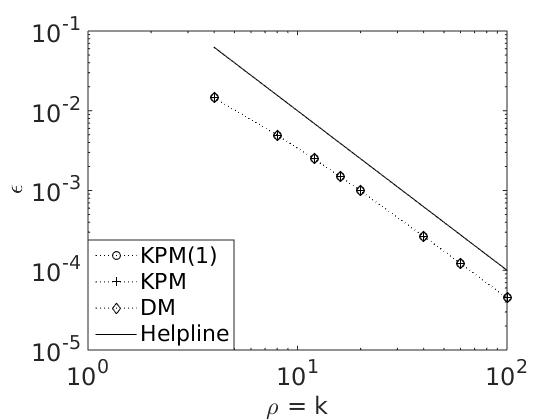
\includegraphics[width=\textwidth]{fig/s1conv1}
                \caption{function \texttt{P1}}
                \label{fig:conv1}
        \end{subfigure}%
~
        \begin{subfigure}[b]{0.45\textwidth}
                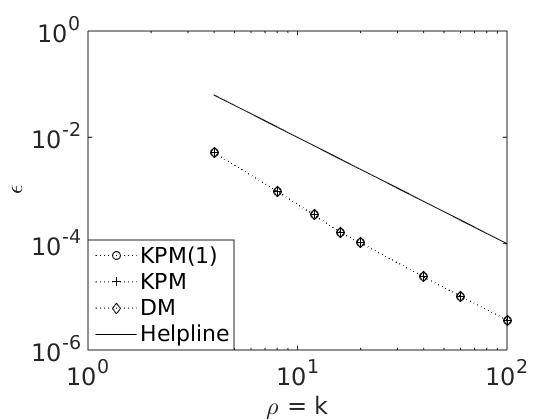
\includegraphics[width=\textwidth]{fig/s2conv2}
                \caption{function \texttt{P2}}
                \label{fig:conv2}
        \end{subfigure}
        \caption{A convergence plot for several methods with $\rho = k$. The helpline shows quadratic convergence.}\label{fig:conv}
\end{figure}
As can be seen from figure \ref{fig:conv}, all method converges quadratically and overlap perfectly, this shows that all method preforms as expected regarding convergence.
%%%%%%%%%%%%%%%%%%%%%%%%%%%%%%%%%%%%%%%%%%%%%%%%%%%%%%%%%%%%%%%%%%%%%%%%%%%%%%%%%%%%%%%%%%%%%%%%%%%%%%%%%%%%%%%%%%%%%%
\section{Choosing restart variable } \label{sec:restvar}
%%%%%%%%%%%%%%%%%%%%%%%%%%%%%%%%%%%%%%%%%%%%%%%%%%%%%%%%%%%%%%%%%%%%%%%%%%%%%%%%%%%%%%%%%%%%%%%%%%%%%%%%%%%%%%%%%%%%%%
\begin{figure}[H]
        \centering
        \begin{subfigure}[b]{0.45\textwidth}
                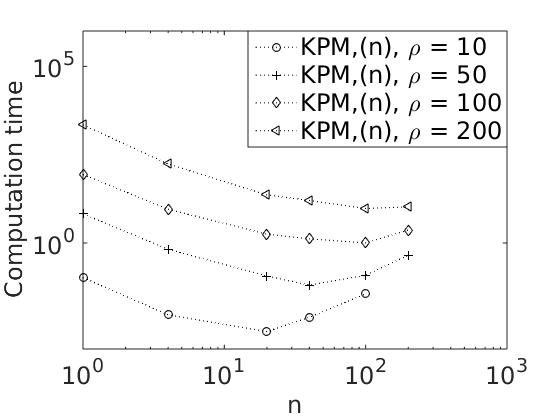
\includegraphics[width=\textwidth]{fig/s9rest1}
                \caption{function \texttt{P1}}
                \label{fig:rest1}
        \end{subfigure}
~
        \begin{subfigure}[b]{0.45\textwidth}
                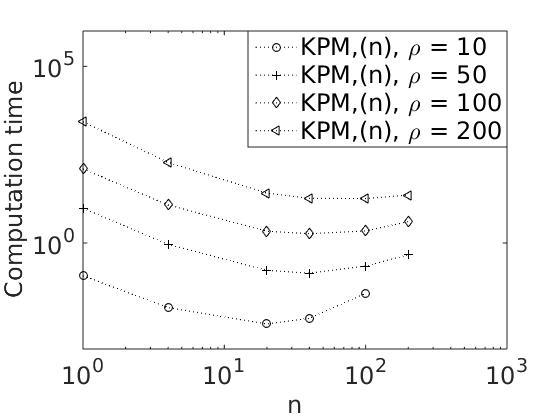
\includegraphics[width=\textwidth]{fig/s10rest2}
                \caption{function \texttt{P2}}
                \label{fig:rest2}
        \end{subfigure}
        \caption{Computation time plotted against restart variable $n$.}\label{fig:rest}
\end{figure}
As can be see from figure \ref{fig:rest}, the optimal restart variable changes as a function of $\rho$ so that larger $\rho$ needs larger $n$ to preform optimally, $n = \rho$ seams to give the smallest computation time for the cases tested. One point is missing from \texttt{KPM}$(n)$, $\rho = 10$, this is because the last point plotted is the same as \texttt{KPM}.  
%%%%%%%%%%%%%%%%%%%%%%%%%%%%%%%%%%%%%%%%%%%%%%%%%%%%%%%%%%%%%%%%%%%%%%%%%%%%%%%%%%%%%%%%%%%%%%%%%%%%%%%%%%%%%%%%%%%%%%
\section{Comparing $\gamma$ and $n$} \label{sec:rrest}
%%%%%%%%%%%%%%%%%%%%%%%%%%%%%%%%%%%%%%%%%%%%%%%%%%%%%%%%%%%%%%%%%%%%%%%%%%%%%%%%%%%%%%%%%%%%%%%%%%%%%%%%%%%%%%%%%%%%%%
\begin{figure}[H]
        \centering
        \begin{subfigure}[b]{0.45\textwidth}
                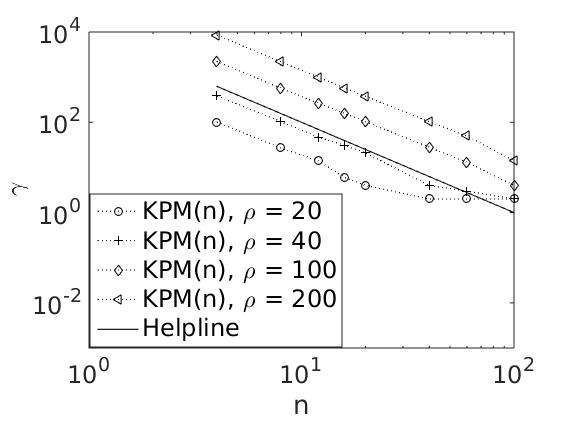
\includegraphics[width=\textwidth]{fig/s3antvsm1}
                \caption{function \texttt{P1}}
                \label{fig:ant1}
        \end{subfigure}%
~
        \begin{subfigure}[b]{0.45\textwidth}
                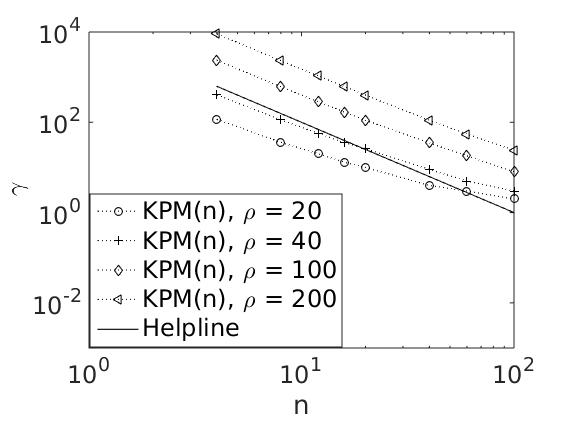
\includegraphics[width=\textwidth]{fig/s4antvsm2}
                \caption{function \texttt{P2}}
                \label{fig:ant2}
        \end{subfigure}
        \caption{The number of restarts, $\gamma$ needed for \texttt{KPM}$(n)$ to converge as a function of the restart variable $n$. The helpline follows $1/n^2$.}\label{fig:ant}
\end{figure}

The helpline from figure \ref{fig:ant} shows that the number of restarts is proportional to $1/n^2$ for all tested cases, if we put this together with the assumption from section \ref{sec:cc} we get that $\gamma$ is proportional to  $m^2/n^2$. Using table \ref{tab:cc} we get that \texttt{KPM}$(\rho)$ has a complexity of $\mathcal{O}(km^2 + m^3)$ for separable $p$, and $\mathcal{O}(km^3 + m^4)$ for non-separable $p$, which is the same as for \texttt{KPM}.\\

We also see that the number of restarts decrease quickest when $n < \rho $, and slower when $n > \rho$. This is the gain we observed in section \ref{sec:restvar}. On each side of $n = \rho$ we can perform better, either by performing fewer restarts with larger matrices, or more restarts with smaller matrices. \\
%%%%%%%%%%%%%%%%%%%%%%%%%%%%%%%%%%%%%%%%%%%%%%%%%%%%%%%%%%%%%%%%%%%%%%%%%%%%%%%%%%%%%%%%%%%%%%%%%%%%%%%%%%%%%%%%%%%%%%
\section{Computation time with different $\rho$} \label{sec:stimem}
%%%%%%%%%%%%%%%%%%%%%%%%%%%%%%%%%%%%%%%%%%%%%%%%%%%%%%%%%%%%%%%%%%%%%%%%%%%%%%%%%%%%%%%%%%%%%%%%%%%%%%%%%%%%%%%%%%%%%%
\begin{figure}[H]
        \centering
        \begin{subfigure}[b]{0.45\textwidth}
                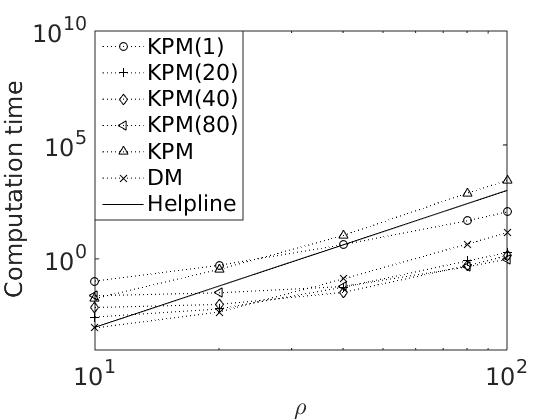
\includegraphics[width=\textwidth]{fig/n5timevsm1}
                \caption{function \texttt{P1}}
                \label{fig:timem1}
        \end{subfigure}%
        ~
        \begin{subfigure}[b]{0.45\textwidth}
                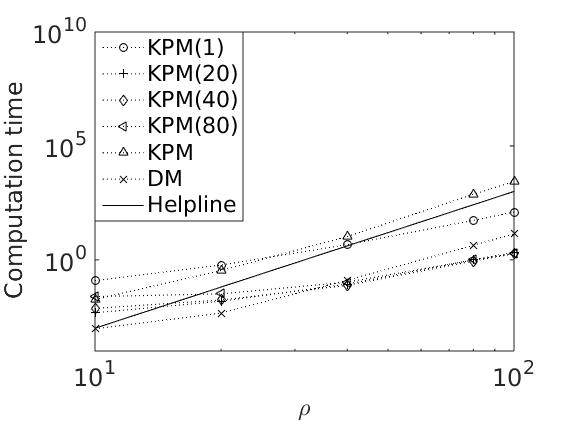
\includegraphics[width=\textwidth]{fig/n6timevsm2}
                \caption{function \texttt{P2}}
                \label{fig:timem2}
        \end{subfigure}
        \caption{A plot of computation time as a function of $\rho$. The helpline increases with $\rho^6 = m^3$.}\label{fig:timem}
\end{figure}
As we can see from figure \ref{fig:timem}, the computation time for \texttt{KPM} increases as expected, while \texttt{DM} and \texttt{KPM}$(n)$ increases slower, perhaps due to MATLAB's efficient inversion algorithm or less memory demand. 
Even more interesting is it that \texttt{KPM}$(n)$ is both asymptotically better, and faster than \texttt{DM} for large $\rho$. Clearly \texttt{KPM}$(n)$ is better in some cases.
%%%%%%%%%%%%%%%%%%%%%%%%%%%%%%%%%%%%%%%%%%%%%%%%%%%%%%%%%%%%%%%%%%%%%%%%%%%%%%%%%%%%%%%%%%%%%%%%%%%%%%%%%%%%%%%%%%%%%%
\section{Computation time with different $k$} \label{sec:stimek}
%%%%%%%%%%%%%%%%%%%%%%%%%%%%%%%%%%%%%%%%%%%%%%%%%%%%%%%%%%%%%%%%%%%%%%%%%%%%%%%%%%%%%%%%%%%%%%%%%%%%%%%%%%%%%%%%%%%%%%
\begin{figure}[H]
        \centering
        \begin{subfigure}[b]{0.45\textwidth}
                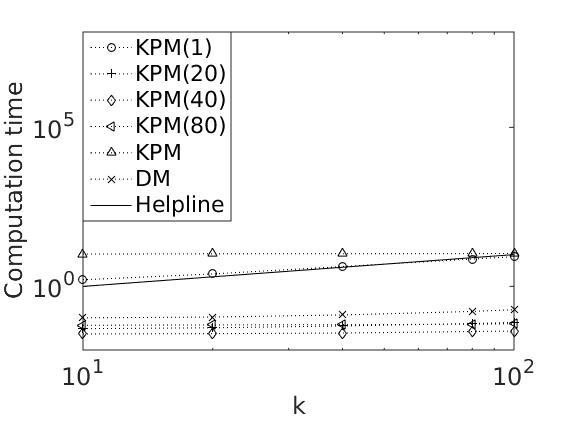
\includegraphics[width=\textwidth]{fig/n7timevsk1}
                \caption{function \texttt{P1}}
                \label{fig:timek1}
        \end{subfigure}%
~
        \begin{subfigure}[b]{0.45\textwidth}
                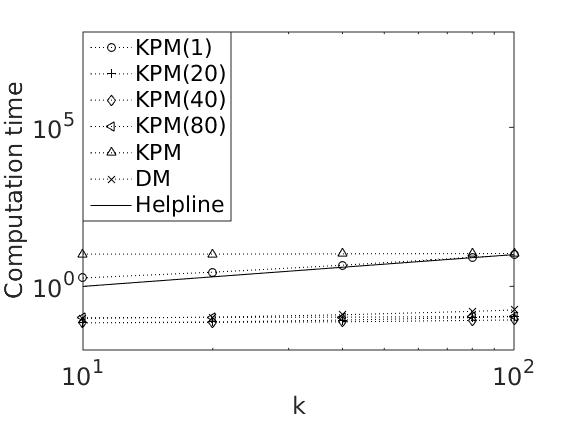
\includegraphics[width=\textwidth]{fig/n8timevsk2}
                \caption{function \texttt{P2}}
                \label{fig:timek2}
        \end{subfigure}
        \caption{A plot of computation time as a function of $k$. The helpline increases with $k$.}\label{fig:timek}
\end{figure}
As we can see from figure \ref{fig:timek}, the computation time for almost all tested methods are constant. The reason is that the time needed for initializing is much greater than the time it takes to integrate. 
The exception is \texttt{KPM}$(1)$, which increases close to linear because relatively more work is done while integrating, due to several restarts. 
We also see that \texttt{KPM}$(n)$ is faster than \texttt{DM} for some $n$, but not asymptotically.

With larger $m$ it is expected that all methods would follow the helpline.
%%%%%%%%%%%%%%%%%%%%%%%%%%%%%%%%%%%%%%%%%%%%%%%%%%%%%%%%%%%%%%%%%%%%%%%%%%%%%%%%%%%%%%%%%%%%%%%%%%%%%%%%%%%%%%%%%%%%%%
\section{Comparing $\delta$, $\gamma$ and $\epsilon$ } \label{sec:div}
%%%%%%%%%%%%%%%%%%%%%%%%%%%%%%%%%%%%%%%%%%%%%%%%%%%%%%%%%%%%%%%%%%%%%%%%%%%%%%%%%%%%%%%%%%%%%%%%%%%%%%%%%%%%%%%%%%%%%%
Remember that $\delta$ is tolerance, $\gamma$ is the number of restarts, and $\epsilon$ is a measure for the error.
\begin{figure}[H]
        \centering
        \begin{subfigure}[b]{0.45\textwidth}
                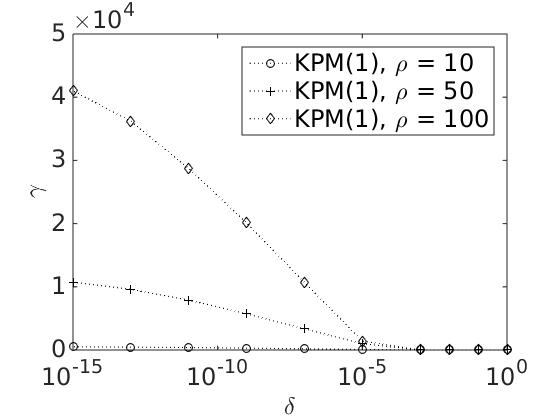
\includegraphics[width=\textwidth]{fig/s13antvstol1m}
                \caption{function \texttt{P1}}
                \label{fig:gammadelta1}
        \end{subfigure}
~
        \begin{subfigure}[b]{0.45\textwidth}
                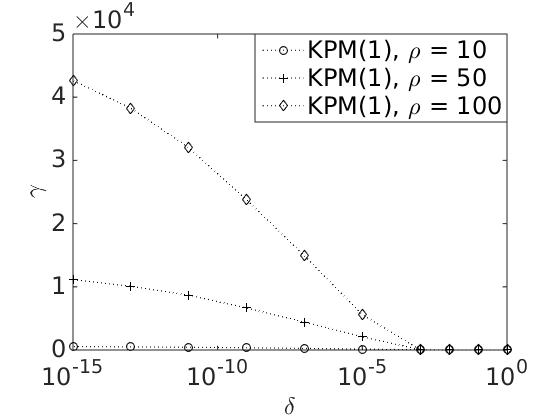
\includegraphics[width=\textwidth]{fig/s14antvstol2m}
                \caption{ function \texttt{P2}}
                \label{fig:gammadelta2}
        \end{subfigure}
        
        \begin{subfigure}[b]{0.45\textwidth}
                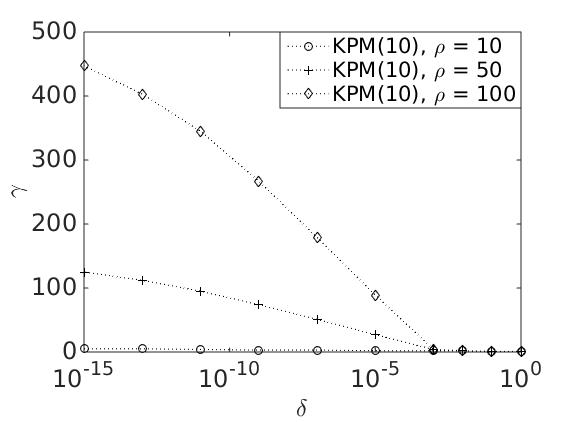
\includegraphics[width=\textwidth]{fig/s13antvstol1m10}
                \caption{function \texttt{P1}}
                \label{fig:gammadelta3}
        \end{subfigure}
~
        \begin{subfigure}[b]{0.45\textwidth}
                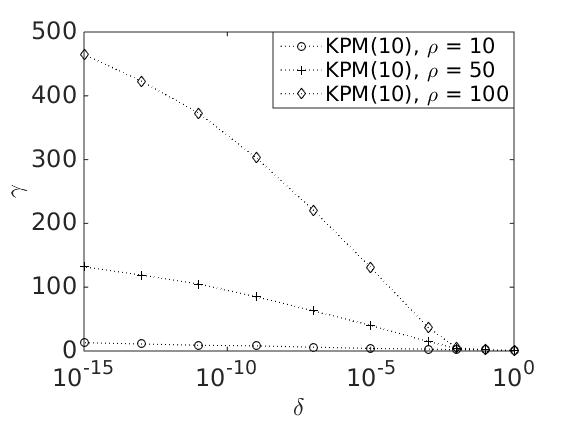
\includegraphics[width=\textwidth]{fig/s14antvstol2m10}
                \caption{ function \texttt{P2}}
                \label{fig:gammadelta4}
        \end{subfigure}
        
        \caption{A plot of $\gamma$ as a function of $\delta$, with several $\rho$ and $n$.} \label{fig:gammadelta}
\end{figure}
We see from figure \ref{fig:gammadelta} that $\gamma$ changes significantly with $\rho$. The figure show a log linear dependence between $\gamma$ and $\delta$, and that $\gamma$ is proportional to $1/n^2$. 
The constant part of the graph where $ 10^{-5}<\delta< {10^0} $ shows that \texttt{KPM}$(1)$ and \texttt{KPM}$(10)$ does too few restarts to gain any accuracy when $\delta$ is too large, this is confirmed by figure \ref{fig:epsilondelta}. 

\begin{figure}[H]
        \centering
        \begin{subfigure}[b]{0.45\textwidth}
                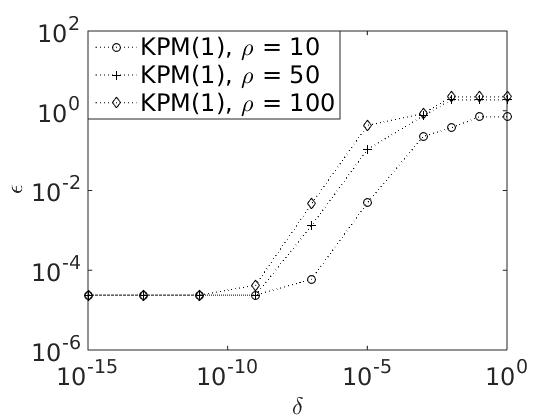
\includegraphics[width=\textwidth]{fig/s15errvstol1m}
                \caption{function \texttt{P1}}
                \label{fig:epsilondelta1}
        \end{subfigure}
~
        \begin{subfigure}[b]{0.45\textwidth}
                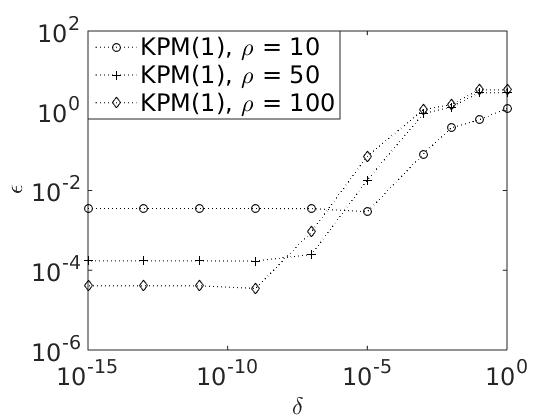
\includegraphics[width=\textwidth]{fig/s16errvstol2m}
                \caption{ function \texttt{P2}}
                \label{fig:epsilondelta2}
        \end{subfigure}
        
        \begin{subfigure}[b]{0.45\textwidth}
                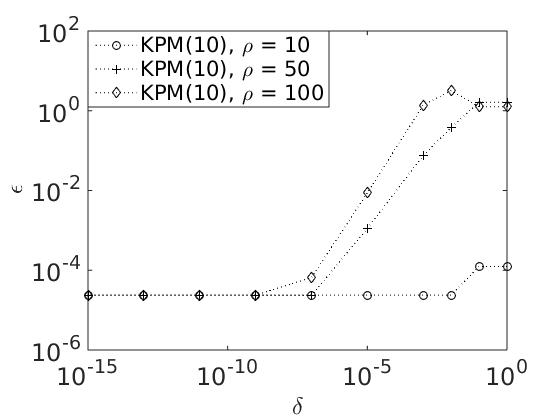
\includegraphics[width=\textwidth]{fig/s15errvstol1m10}
                \caption{function \texttt{P1}}
                \label{fig:epsilondelta3}
        \end{subfigure}
~
        \begin{subfigure}[b]{0.45\textwidth}
                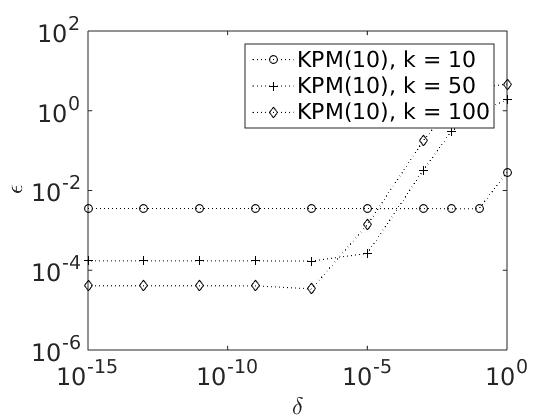
\includegraphics[width=\textwidth]{fig/s16errvstol2m10}
                \caption{ function \texttt{P2}}
                \label{fig:epsilondelta4}
        \end{subfigure}
        
        \caption{A plot of $\epsilon$ as a function of $\delta$, with several $\rho$ and $n$.} \label{fig:epsilondelta}
\end{figure}
Figure \ref{fig:epsilondelta} shows $\epsilon$ as a function of $\delta$. In figure \ref{fig:epsilondelta1} and \ref{fig:epsilondelta3} all graphs has obtained the threshold precision possible with $k=40$. In
figure \ref{fig:epsilondelta2} and \ref{fig:epsilondelta4} the precision possible with the different $\rho$-s are obtained. It seams that the maximum precision is attained faster with larger $n$, this makes sense because if $n = m$, we should not need to restart in order to get threshold precision. This was also confirmed by figure \ref{fig:gammadelta}, where \texttt{KPM}$(10)$ needed fewer restarts than \texttt{KPM}$(1)$ to converge. 
%There is no reason this was not performed with other than $n = 1$ except for laziness. \\
%!!!!!!!!!!!!!!!!!!!!!!!!!Arg, jeg må lage nye figurer for andre $n$!!!!!!!!!!!!!!!!!!!!!!!!!!!!!!!!!!\\
%!!!!!!!!!!!!!!!!Her kan burde skrive noe om hvor bra KPM$(n)$ uten restart ville vært!!!!!!!!!!!!!!!!\\
%!!!!!!!!!!!!!!!!!!!!!Fjern alle forekomster av ordet "shows" fra avsnittet!!!!!!!!!!!!!!!!!!!!!!!!!!!!\\
%!!!!!!!!!!!!!!!!!!!!!Forklare hva alle variablene er over alt!!!!!!!!!!!!!!!!!!!!!!!!!!\\
%!!!!!!!!!!!!!!!!!!!!!Skrive hvorfor vi ikke har med noe annet enn KPM$(1)$!!!!!!!!!!!!!!!!!!\\
%!!!!!!!!!!!!!!!!!!!!!!!!!!!Går videre så jeg ikke trenger å lage nye figurer med en gang!!!!!!!!!!!!!!!!!!!!!!!!!!\\
%Figure \ref{fig:errant} and \ref{fig:errtolk} shows how $\gamma$ and $\epsilon$ scales with $\delta$. Figure \ref{fig:errtol1} has reached to threshold precision with $k = 40$. Both figures shows a loglinear dependence between $\gamma$ and $\delta$. The figures also shows the importance of choosing an appropriate $\delta$. A lot of time can be saved by choosing $\delta$ larger, but precision is lost if $\delta$ is to large.
\begin{figure}[H]
        \centering
        \begin{subfigure}[b]{0.45\textwidth}
                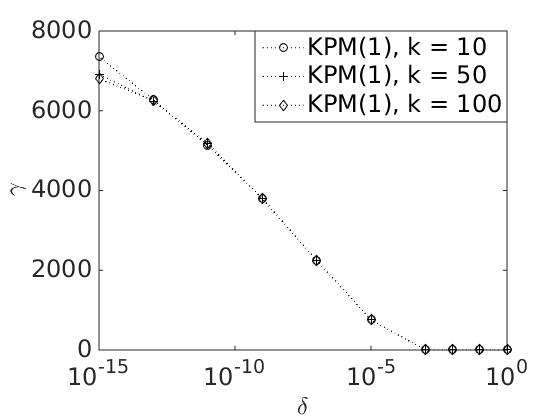
\includegraphics[width=\textwidth]{fig/s20antvstol1k}
                \caption{function \texttt{P1}}
                \label{fig:gammadeltak1}
        \end{subfigure}
~
        \begin{subfigure}[b]{0.45\textwidth}
                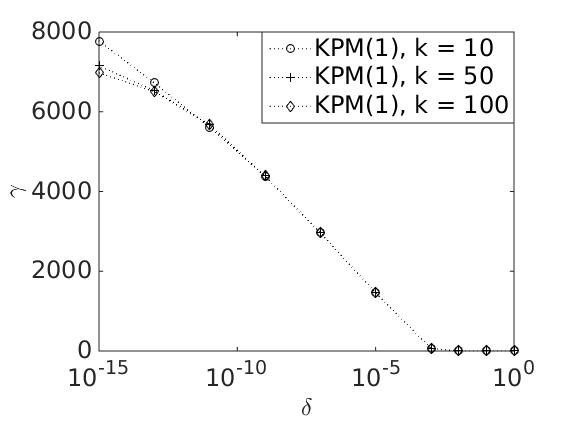
\includegraphics[width=\textwidth]{fig/s21antvstol2k}
                \caption{ function \texttt{P2}}
                \label{fig:gammadeltak2}
        \end{subfigure}
                \begin{subfigure}[b]{0.45\textwidth}
                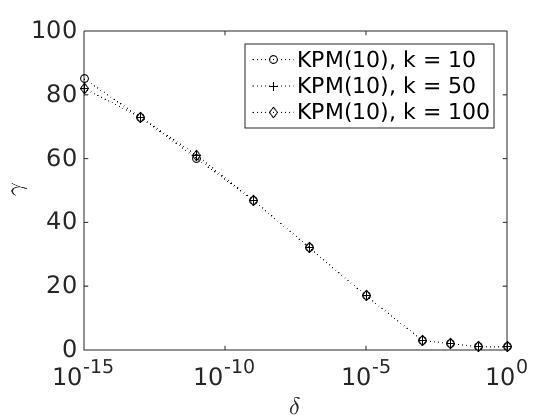
\includegraphics[width=\textwidth]{fig/s20antvstol1k10}
                \caption{function \texttt{P1}}
                \label{fig:gammadeltak3}
        \end{subfigure}
~
        \begin{subfigure}[b]{0.45\textwidth}
                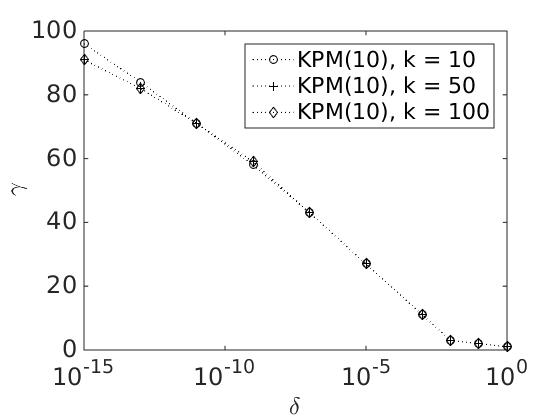
\includegraphics[width=\textwidth]{fig/s21antvstol2k10}
                \caption{ function \texttt{P2}}
                \label{fig:gammadeltak4}
        \end{subfigure}
        \caption{A plot of $\gamma$ as a function of $\delta$, with several $k$ and $n$.} \label{fig:gammadeltak}
\end{figure}
Figure \ref{fig:gammadeltak} shows that $\gamma$ is nearly independent of $k$. The figures also shows the log linear dependence between $\delta$ and $\gamma$. \\



\begin{figure}[H]
        \centering
        \begin{subfigure}[b]{0.45\textwidth}
                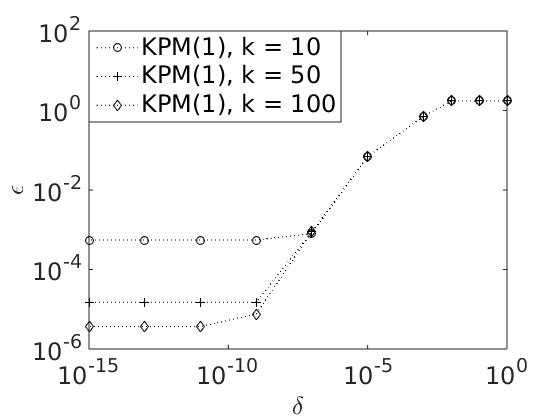
\includegraphics[width=\textwidth]{fig/s22errvstol1k}
                \caption{function \texttt{P1}}
                \label{fig:epsilondelta1k}
        \end{subfigure}
~
        \begin{subfigure}[b]{0.45\textwidth}
                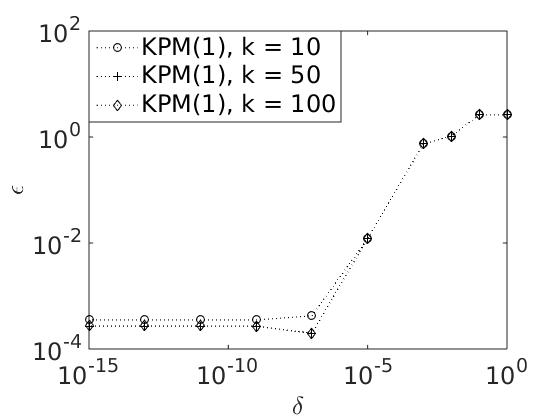
\includegraphics[width=\textwidth]{fig/s23errvstol2k}
                \caption{ function \texttt{P2}}
                \label{fig:epsilondelta2k}
        \end{subfigure}
                \begin{subfigure}[b]{0.45\textwidth}
                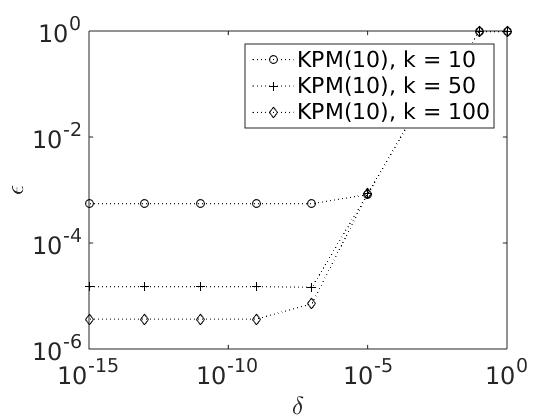
\includegraphics[width=\textwidth]{fig/s22errvstol1k10}
                \caption{function \texttt{P1}}
                \label{fig:epsilondelta3k}
        \end{subfigure}
~
        \begin{subfigure}[b]{0.45\textwidth}
                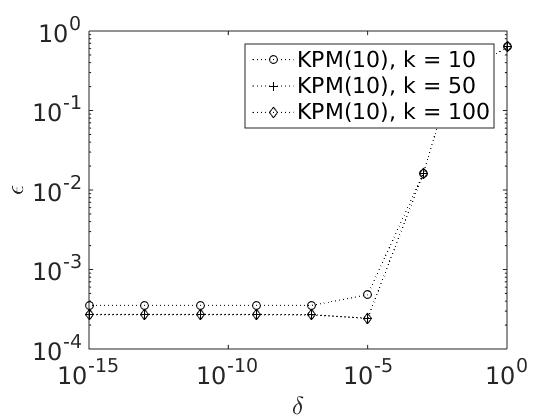
\includegraphics[width=\textwidth]{fig/s23errvstol2k10}
                \caption{ function \texttt{P2}}
                \label{fig:epsilondelta4k}
        \end{subfigure}
        \caption{A plot of $\epsilon$ as a function of $\delta$, with several $k$ and $n$.} \label{fig:epsilondeltak}
\end{figure}
Figure \ref{fig:epsilondeltak} shows much the same as figure \ref{fig:epsilondelta}. Maximum precision for different $k$-s are shown in figure \ref{fig:epsilondelta1k} and \ref{fig:epsilondelta3k}.
Threshold precision for $\rho = 40$ is obtained in figure \ref{fig:epsilondelta2k} and \ref{fig:epsilondelta4k}, but not for the graph where $k = 10$, this is the precision possible with $k=10$. Again $\epsilon$ converges faster for \texttt{KPM}$(10)$ than \texttt{KPM}$(1)$. \\

We see that there is no gain in precision with increasing one of either $\rho$ or $k$ or decreasing $\delta$ without changing the others appropriately. \\

%Before the constant part, $\epsilon$ is decided by $\delta$ alone. 
In all cases a lot of time can be saved by choosing $\delta$ appropriate. If $\delta$ is to large we get inaccurate answers, if $\delta$ is to small we perform to many restarts to use the algorithm efficiently. There does not seam to be a simple rule to choose $\delta$, since the results for \texttt{P1} and \texttt{P2} differs. The rule we will use is to start at $\delta=10^{-3}$ with $\rho = k = 10$, and decrease $\delta$ with two order of magnitude each time $k$ and $\rho$ is doubled. The reason for this rule is perhaps easier to understand when looking at figure \ref{fig:conv}. The reason that $\delta$ decreases two orders of magnitude each time $m$ and $k$ is doubled is that $A$ and trapezoidal rule are second order approximations. Figure \ref{fig:siste} shows how the error converges when this is the case, clearly this rule assures that $\delta$ is small enough.

\begin{figure}[H]
        \centering
        \begin{subfigure}[b]{0.45\textwidth}
                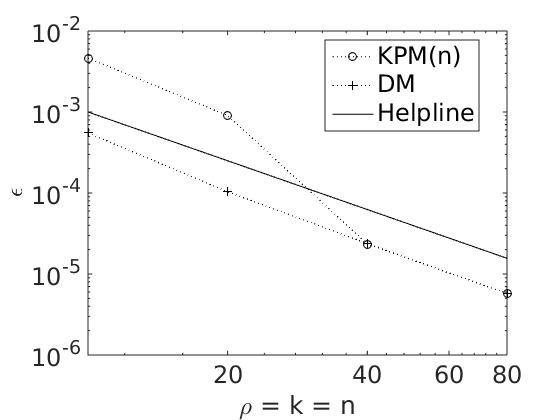
\includegraphics[width=\textwidth]{fig/sisteplot1}
                \caption{function \texttt{P1}}
                \label{fig:siste1}
        \end{subfigure}
~
        \begin{subfigure}[b]{0.45\textwidth}
                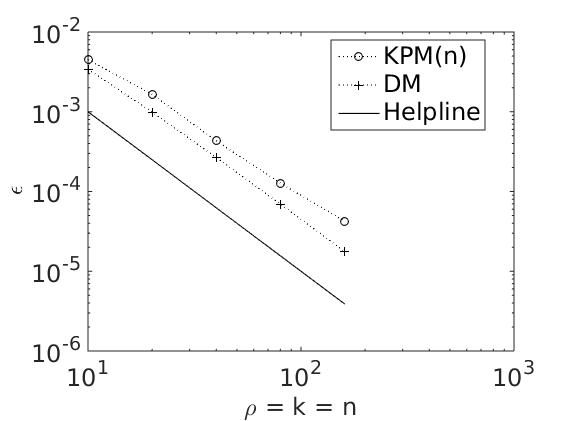
\includegraphics[width=\textwidth]{fig/sisteplot2}
                \caption{ function \texttt{P2}}
                \label{fig:siste2}
        \end{subfigure}
        \caption{A plot of $\epsilon$ where $\delta$, $k$, $\rho$ and $n$ follows this rule: Start with $\delta=10^{-3}$, $\rho = k = n = 10$ and decrease $\delta$ with two order of magnitude each time $k$, $\rho$ and $n$ is doubled. \texttt{DM} Shows how it converged when $\delta = 10^{-15}$. The helpline shows quadratic convergence.} \label{fig:siste}
\end{figure}


%%%%%%%%%%%%%%%%%%%%%%%%%%%%%%%%%%%%%%%%%%%%%%%%%%%%%%%%%%%%%%%%%%%%%%%%%%%%%%%%%%%%%%%%%%%%%%%%%%%%%%%%%%%%%%%%%%%%%%
\chapter{Results for non-separable $p$} \label{sec:para}%%%%%%%%%%%%%%%%%%%%%%%%%%%%%%%%%%%%%%%%%%%%%%%%%%%%%%%%%%%%%
%%%%%%%%%%%%%%%%%%%%%%%%%%%%%%%%%%%%%%%%%%%%%%%%%%%%%%%%%%%%%%%%%%%%%%%%%%%%%%%%%%%%%%%%%%%%%%%%%%%%%%%%%%%%%%%%%%%%%%
%We will now use what we learned from the previous section in a parallel setting with $p$ non-separable and see if we can make KPM outperform DM.

We now assume that $p$ is non-separable, so that we need to solve $m$ independent problems when using KPM. Several processing units will be used when possible. \\% . We will make use of several processing units, together with what we learned in section \ref{sec:seri} to see if we can make KPM outperform DM.

We start by showing correctness of the methods with a convergence plot in section \ref{sec:pconv}, and proceed with looking into speedup and parallel efficiency in section \ref{sec:speed}. We end by investigating how computation time for the best possible case of KPM compares to DM in section \ref{sec:compare}. 

%%%%%%%%%%%%%%%%%%%%%%%%%%%%%%%%%%%%%%%%%%%%%%%%%%%%%%%%%%%%%%%%%%%%%%%%%%%%%%%%%%%%%%%%%%%%%%%%%%%%%%%%%%%%%%%%%%%%%%
\section{Convergence} \label{sec:pconv}
%%%%%%%%%%%%%%%%%%%%%%%%%%%%%%%%%%%%%%%%%%%%%%%%%%%%%%%%%%%%%%%%%%%%%%%%%%%%%%%%%%%%%%%%%%%%%%%%%%%%%%%%%%%%%%%%%%%%%%
\begin{figure}[H]
        \centering
        \begin{subfigure}[b]{0.45\textwidth}
                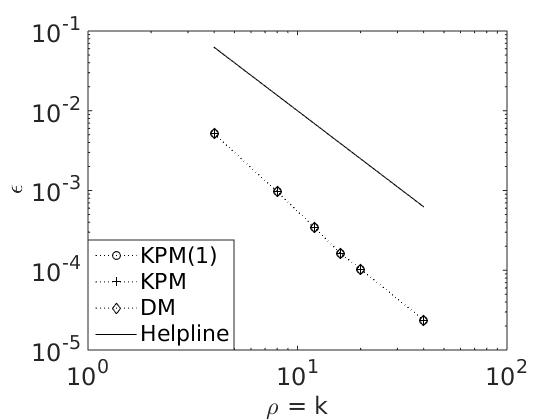
\includegraphics[width=\textwidth]{fig/p1conv1}
                %\includegraphics[width=\textwidth]{test}
                \caption{function \texttt{P1}}
                \label{fig:conv1p}
        \end{subfigure}%
        ~
        \begin{subfigure}[b]{0.45\textwidth}
                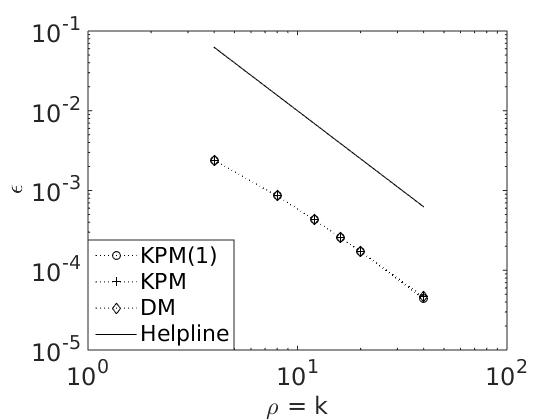
\includegraphics[width=\textwidth]{fig/p2conv2}
                %\includegraphics[width=\textwidth]{test}
                \caption{function \texttt{P3}}
                \label{fig:conv2p}
        \end{subfigure}
        \caption{A convergence plot for several methods with $\rho = k$. The helpline shows quadratic convergence.}\label{fig:convp}
\end{figure}
As can be seen from figure \ref{fig:convp}, all methods converges quadratically and identically, as in section \ref{sec:sconv}. All methods therefore perform as expected regarding convergence.
%%%%%%%%%%%%%%%%%%%%%%%%%%%%%%%%%%%%%%%%%%%%%%%%%%%%%%%%%%%%%%%%%%%%%%%%%%%%%%%%%%%%%%%%%%%%%%%%%%%%%%%%%%%%%%%%%%%%%%
\section{Speedup} \label{sec:speed}
%%%%%%%%%%%%%%%%%%%%%%%%%%%%%%%%%%%%%%%%%%%%%%%%%%%%%%%%%%%%%%%%%%%%%%%%%%%%%%%%%%%%%%%%%%%%%%%%%%%%%%%%%%%%%%%%%%%%%%
\begin{figure}[H]
        \centering
        \begin{subfigure}[b]{0.45\textwidth}
                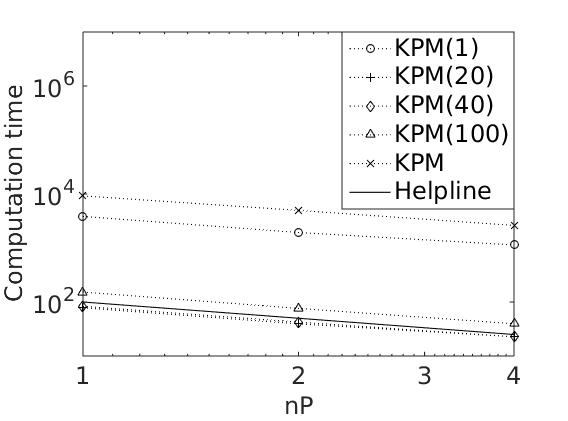
\includegraphics[width=\textwidth]{fig/u1para1}
                %\includegraphics[width=\textwidth]{test}
                \caption{function \texttt{P1}}
                \label{fig:speed1}
        \end{subfigure}%
        ~
        \begin{subfigure}[b]{0.45\textwidth}
                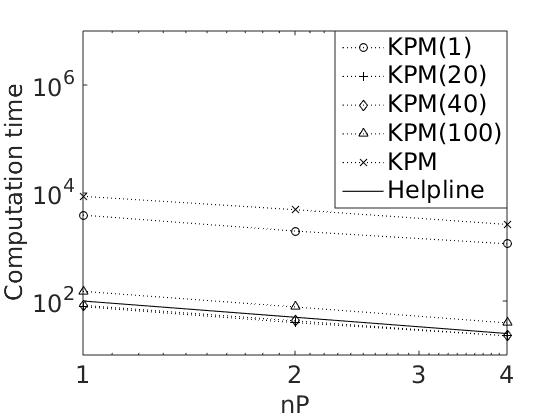
\includegraphics[width=\textwidth]{fig/u2para2}
                %\includegraphics[width=\textwidth]{test}
                \caption{function \texttt{P3}}
                \label{fig:speed2}
        \end{subfigure}
        \caption{Computation time plotted against different number of processors, for several methods. The helpline shows perfect speedup.}\label{fig:speed}

\end{figure}

\begin{table}[H]
\centering
\begin{tabular}{l | l l | l l}
%\textrhoticity Skriv påskeegg her!
%$\Pluto$
%\textrhoticity
%$\textrhoticity$
%\textpalhookvar
%$\textpalhookvar$
%\closedniomega $\closedniomega$
%\underwedge $\underwedge$
%$\pluto$ $\Pluto$
%$\libra$
$\neptune$ %$\Neptune$
%$\llcorner$
 &\texttt{P1} & & \texttt{P3} & \\
&\texttt{nP = 2} & \texttt{nP = 4} & \texttt{nP = 2} & \texttt{nP = 4} \\
\hline
KPM & 1.8556  &  3.5234 & 1.7702&    3.3193\\
KPM$(1)$ & 1.9858  &  3.3740 & 1.9725&    3.3924\\
KPM$(20)$ & 1.9883  &  3.4525 & 1.9756&    3.4547\\
KPM$(40)$ & 1.9619  &  3.6667 & 1.9352&   3.6642\\
KPM$(100)$ & 2.0083  &  3.8618 & 1.9437&    3.8362\\
\end{tabular}
\caption{Speedup for several cases of KPM.}
\label{tab:speedup}
\end{table}

\begin{table}[H]
\centering
\begin{tabular}{l | l l | l l}
&\texttt{P1} & & \texttt{P3} & \\
&\texttt{nP = 2} & \texttt{nP = 4} & \texttt{nP = 2} & \texttt{nP = 4} \\
\hline
KPM & 0.9278  &  0.8809 & 0.8851&    0.8298\\
KPM$(1)$ &  0.9929  &  0.8435 & 0.9862 &   0.8481\\
KPM$(20)$ & 0.9942  &  0.8631 & 0.9878&    0.8637\\
KPM$(40)$ & 0.9809  &  0.9167 & 0.9676&    0.9160\\
KPM$(100)$ & 1.0042  &  0.9655 & 0.9719&    0.9591\\
\end{tabular}
\caption{Parallel efficiency for several cases of KPM. }
\label{tab:eff}
\end{table}

From figure \ref{fig:speed} together with table \ref{tab:speedup} and \ref{tab:eff} we can observe the gain by using several processing units. Parallel efficiency and speedup is high for all cases of KPM tested here, it is definitely efficient to use several processing units on this type of problem. \\%All values of $n < m$ seams to give good parallel gain. \\

These experiments was only done with $m = k = 40$, this is because the experiments took much time on this computer. I see no reason why parallel gain should change significantly with other $m$ or $k$. 

%%%%%%%%%%%%%%%%%%%%%%%%%%%%%%%%%%%%%%%%%%%%%%%%%%%%%%%%%%%%%%%%%%%%%%%%%%%%%%%%%%%%%%%%%%%%%%%%%%%%%%%%%%%%%%%%%%%%%%
\section{Comparison} \label{sec:compare}
%%%%%%%%%%%%%%%%%%%%%%%%%%%%%%%%%%%%%%%%%%%%%%%%%%%%%%%%%%%%%%%%%%%%%%%%%%%%%%%%%%%%%%%%%%%%%%%%%%%%%%%%%%%%%%%%%%%%%%
\begin{figure}[H]
        \centering
        \begin{subfigure}[b]{0.45\textwidth}
                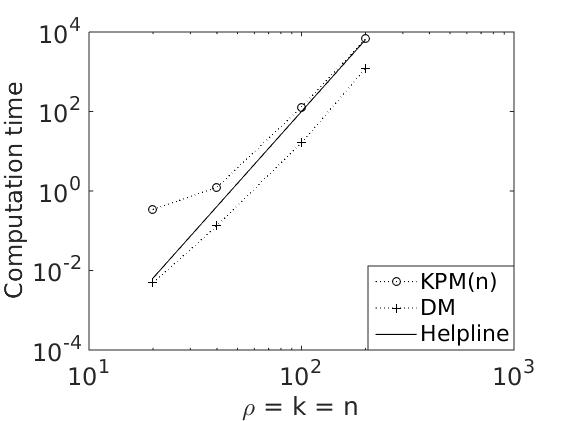
\includegraphics[width=\textwidth]{fig/comp2}
                \caption{function \texttt{P1}}
                \label{fig:c1comp1m}
        \end{subfigure}%
        ~
        \begin{subfigure}[b]{0.45\textwidth}
                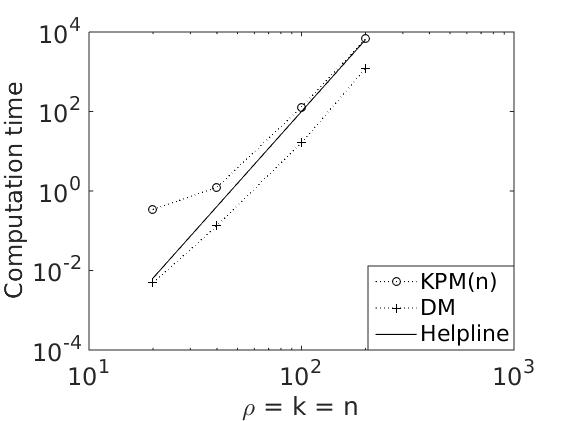
\includegraphics[width=\textwidth]{fig/comp2}
                \caption{function \texttt{P3}}
                \label{fig:c2comp2m}
        \end{subfigure}
        \caption{A plot of the computation time for KPM$(n)$ and DM. We have used the values $n = \rho = k$. $\delta = 10^{-3}$ for the first point and decreases with two orders of magnitude for each additional point. Assume $\texttt{nP} = 4$ for KPM$(n)$ and $\texttt{nP} = 1$ for DM. These values are choosen to make KPM$(n)$ perform as efficiently as possible. The helpline increases with $\rho^6 = m^3$.}\label{fig:comp}
\end{figure}
From figure \ref{fig:comp} it is clear that DM is better in all cases simulated, but KPM$(n)$ is not far behind. We know from section \ref{sec:stimem} and \ref{sec:stimek} that one iteration of KPM$(n)$ is faster than DM, we therefore conclude that with enough processing units KPM$(\rho)$ would have been faster than DM. \\

The other important thing to note here is that computation time for KPM$(n)$ does not increase faster than for DM. It is difficult to say what would happen with larger $\rho$ or $k$, but they would probably follow the helpline.\\

The first point of KPM$(n)$ in both figures are very high compared to the trend, perhaps the problem size is to small to be used efficiently with several processing units. 

%%%%%%%%%%%%%%%%%%%%%%%%%%%%%%%%%%%%%%%%%%%%%%%%%%%%%%%%%%%%%%%%%%%%%%%%%%%%%%%%%%%%%%%%%%%%%%%%%%%%%%%%%%%%%%%%%%%%%%
\chapter{Discussion and conclusion}%%%%%%%%%%%%%%%%%%%%%%%%%%%%%%%%%%%%%%%%%%%%%%%%%%%%%%%%%%%%%%%%%%%%%%%%%%%%%%%%%%
%%%%%%%%%%%%%%%%%%%%%%%%%%%%%%%%%%%%%%%%%%%%%%%%%%%%%%%%%%%%%%%%%%%%%%%%%%%%%%%%%%%%%%%%%%%%%%%%%%%%%%%%%%%%%%%%%%%%%%

Theoretically all methods perform about the same when $p$ is separable. If $p$ is not separable \texttt{DM} has a clear advantage. If we assume that $\gamma$ is proportional to $m^2/n^2$, which we concluded in section \ref{sec:rrest}, and use $n = \rho$ as suggested in section \ref{sec:restvar}, we get that \texttt{KPM}$(\rho)$ performs asymptotically equal to \texttt{KPM}. This follows from table \ref{tab:cc}. \\

When $p$ is separable, the results from section \ref{sec:stimem} and \ref{sec:stimek} shows that \texttt{KPM}$(n)$ is faster and asymptotically better than \texttt{DM}. This contradicts the results from theoretical complexity, and might be due to the smaller memory demand. \\

The reason for the high parallel performance in section \ref{sec:speed} is the natural independence in the method. The only communication needed between processors is when adding results, this can be done in $\log_2(\texttt{nP})$ additions. Note that a good restart variable also gives a good problem size to use with parallel computations. \\

Regarding convergence all methods can perform equally well, the drawback is the need to choose an appropriate $\delta$ for \texttt{KPM}$(n)$. With a larger $\delta$ \texttt{KPM}$(n)$ is less accurate, but with smaller $\delta$ we restart too many times, making the methods inefficient. The rule of thumbs is start at $\delta=10^{-3}$ with $\rho = k = n = 10$, and decrease $\delta$ with one order of magnitude each time $\rho = k = n$ is doubled. \\

Table \ref{tab:mr} shows that \texttt{KPM}$(n)$ for $n \leq \rho$ uses the least amount of memory. This is one of the main reasons to use KPM instead of \texttt{DM} on this type of problems. \\

In section \ref{sec:compare} we used what we had learned about $\gamma$, $n$ and $\delta$ to make \texttt{KPM}$(n)$ run as fast as possible with $p$ non-separable. \texttt{DM} was faster than \texttt{KPM}$(\rho)$, but not asymptotically, as suggested by table \ref{tab:cc}. With more processors \texttt{KPM}$(n)$ would have been faster because of the high parallel efficiency and the low cost of solving each of the $m$ independent problems. \\

%that KPM$(\rho)$ has the same complexity as KPM. So if $p$ is separable all methods perform equally well, if $p$ is non-separable DM requires fewer operations. 

 %if $p$ is separable. If $p$ is not separable DM has again an advantage over KPM and KPM$(n)$. \\



It is worth noting that \texttt{DM} did not work when $\rho>300$ due to memory shortage, while \texttt{KPM}$(n)$ had no problem with $\rho = 1000$ and $n = 40$. \\

%%%%%%%%%%%%%%%%%%%%%%%%%%%%%%%%%%%%%%%%%%%%%%%%%%%%%%%%%%%%%%%%%%%%%%%%%%%%%%%%%%%%%%%%%%%%%%%%%%%%%%%%%%%%%%%%%%%%%%
\chapter*{Further work}%%%%%%%%%%%%%%%%%%%%%%%%%%%%%%%%%%%%%%%%%%%%%%%%%%%%%%%%%%%%%%%%%%%%%%%%%%%%%%%%%%%%%%%%%%%%%%
%%%%%%%%%%%%%%%%%%%%%%%%%%%%%%%%%%%%%%%%%%%%%%%%%%%%%%%%%%%%%%%%%%%%%%%%%%%%%%%%%%%%%%%%%%%%%%%%%%%%%%%%%%%%%%%%%%%%%%
To obtain better results KPM should be implemented in a more parallel friendly language, as for example \texttt{C}. It would also be a benefit to use a large computer, making it easier to get data with larger $\rho$ and $k$.

It would also be interesting to see how KPM could be used to solve other equations than the heat equation.
%%%%%%%%%%%%%%%%%%%%%%%%%%%%%%%%%%%%%%%%%%%%%%%%%%%%%%%%%%%%%%%%%%%%%%%%%%%%%%%%%%%%%%%%%%%%%%%%%%%%%%%%%%%%%%%%%%%%%%
\chapter*{My code}%%%%%%%%%%%%%%%%%%%%%%%%%%%%%%%%%%%%%%%%%%%%%%%%%%%%%%%%%%%%%%%%%%%%%%%%%%%%%%%%%%%%%%%%%%%%%%%%%%%
%%%%%%%%%%%%%%%%%%%%%%%%%%%%%%%%%%%%%%%%%%%%%%%%%%%%%%%%%%%%%%%%%%%%%%%%%%%%%%%%%%%%%%%%%%%%%%%%%%%%%%%%%%%%%%%%%%%%%%

If you are interested in any of the code used here you can find it at: \\
\emph{https://github.com/sindreka/Prosjektoppgave}

% Include more chapters as required.
%%=========================================
%\appendix
%% !TEX encoding = UTF-8 Unicode
%!TEX root = thesis.tex
% !TEX spellcheck = en-US
%%=========================================

\chapter{Acronyms}
\begin{description}
\item[FTA] Fault tree analysis
\item[MTTF] Mean time to failure
\item[RAMS] Reliability, availability, maintainability, and safety
\end{description}
%% !TEX encoding = UTF-8 Unicode
%!TEX root = thesis.tex
% !TEX spellcheck = en-US
%%=========================================

\chapter{Additional Information}
This is an example of an Appendix. You can write an Appendix in the same way as a chapter, with sections, subsections, and so on.

%%=========================================
\section{Introduction}

%%=========================================
\subsection{More Details}
% Include more appendices as required.
%%=========================================
\bibliographystyle{apa}
\addcontentsline{toc}{chapter}{\bibname}
\bibliography{refs}  
%%=========================================
%% !TEX encoding = UTF-8 Unicode
%!TEX root = thesis.tex
% !TEX spellcheck = en-US

%This is the Curriculum Vitae
%%=========================================
\addcontentsline{toc}{chapter}{Curriculum Vitae}
\chapter*{Curriculum Vitae}
\hrule
\begin{minipage}[t]{0.65\linewidth}
\begin{tabular}{ll}
Name: & \textbf{Your Name}\\
Gender: & Female\\
Date of birth: & 1. January 1995\\
Address: & Nordre gate 1, N--7005 Trondheim \\
Home address: & King's road 1, 4590 Vladivostok, Senegal\\
Nationality:    & English \\
Email (1): & your.name@stud.ntnu.no\\
Email (2): & yourname@gmail.com\\
Telephone: & +47 12345678\\
\end{tabular} 
\end{minipage}\hfill
\begin{minipage}[t]{0.25\linewidth}
\includegraphics[scale=0.3]{fig/me}\\[1pc] Your picture
\end{minipage}
\hrule

%%=========================================
\section*{Language Skills}
Describe which languages you speak and/or write. Specify your skills in each language.

%%=========================================
\section*{Education}
\begin{itemize}
\item School 1
\item School 2
\item School 3
\end{itemize}

%%=========================================
\section*{Computer Skills}
\begin{itemize}
\item Program 1
\item Program 2
\item Program 3
\end{itemize}

%%=========================================
\section*{Experience}
\begin{itemize}
\item Job 1
\item Job 2
\item Job 3
\end{itemize}

%%=========================================
\section*{Hobbies and Other Activities}         % Your curriculum Vitae     
%%=============================================

\end{document}
